\begin{center}
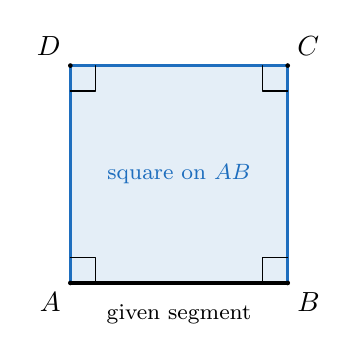
\begin{tikzpicture}[scale=1.15, line cap=round, line join=round]
  \definecolor{euclidblue}{RGB}{30,110,190}
  \coordinate (A) at (0,0);
  \coordinate (B) at (2.4,0);
  \coordinate (C) at (2.4,2.4);
  \coordinate (D) at (0,2.4);
  \fill[euclidblue!12] (A)--(B)--(C)--(D)--cycle;
  \draw[very thick, euclidblue] (A)--(B)--(C)--(D)--cycle;
  \draw[very thick] (A)--(B);
  \draw (0.28,0)--(0.28,0.28)--(0,0.28);
  \draw (2.12,0)--(2.12,0.28)--(2.4,0.28);
  \draw (2.12,2.4)--(2.12,2.12)--(2.4,2.12);
  \draw (0.28,2.4)--(0.28,2.12)--(0,2.12);
  \foreach \p/\pos in {A/below left,B/below right,C/above right,D/above left}{
    \fill (\p) circle (0.026);
    \node[\pos] at (\p) {$\p$};
  }
  \node[font=\footnotesize] at (1.2,-0.35) {given segment};
  \node[euclidblue, font=\footnotesize] at (1.2,1.2) {square on $AB$};
\end{tikzpicture}
\end{center}
